%!TEX root=main.tex
\begin{section}{Performance results}
	\label{sec:performance}
	\begin{subsection}{Experimental setup}
		\label{sec:setup}
		All experiments are run on two socket (2S) 2.40GHz Intel\textregistered{} Xeon\textregistered{} Gold 6148 processors. There are 20 cores per socket with 2-way hardware multi-threading. On-chip L1 data cache is 32KB. L2 and L3 caches are 1MB and 28MB respectively. For multi-node experiments, we used up to 64 Intel\textregistered{} Xeon\textregistered{} Gold connected via 100gigabits/second Intel\textregistered{} OP Fabric. Each server has 192GB physical memory and a 1.6TB Intel SSD storage drive. The M-CNN topology was added to the standard benchmarking scripts \cite{GoogleTPU} to leverage instantiation mechanisms of distributed workers. Gradient synchronization between the workers was done using Horovod, an MPI-based communication library for deep learning training \cite{Horovod}. In our experiments, we used TensorFlow 1.9.0, Horovod 0.13.4, Python 2.7.5 and OpenMPI 3.0.0.
	\end{subsection}
	\begin{subsection}{Scaling up TTT in One Node with Dataset A}
		\label{sec:scaleup}
\noindent We first performed a sweep of batch sizes from 4, 8, 16, 32 and 64 to check how fast we can converge on one CPU server. We acheived convergence in 5hrs 31mins with batch size = 32. The resulting throughput and memory consumed are shown in Figure \ref{fig:multiworker} \subref{fig:singlenodethroughput1w} and Figure \ref{fig:multiworker} \subref{fig:singlenodememutil1w}, respectively. As shown in the latter figure, the memory footprint of M-CNN far exceeds the activation size of the model. For example, in case of batch size of 32, total memory used is 47.5GB which is 4x larger than activation size of 11GB as calculated in \autoref{fig:batchsize}. The additional memory is allocated by TensorFlow to instantiate temporary variables used in both forward and backward propagation, buffers to read data and others operations. Due to these overheads, memory utilization of M-CNN is prohibitively high and it is difficult to scale to large batch sizes when memory in the system is limited. \\
		\begin{figure}[t]
	\centering
	\begin{subfigure}[t]{0.45\textwidth}
		\centering
		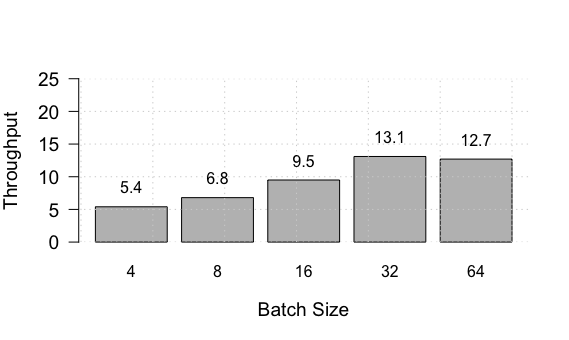
\includegraphics[width=\textwidth]{wgrid_figure3a.png}
		\caption{Throughput (in images/sec) -- 1 worker}
		\label{fig:singlenodethroughput1w}
	\end{subfigure} 
	\begin{subfigure}[t]{0.45\textwidth}
		\centering
		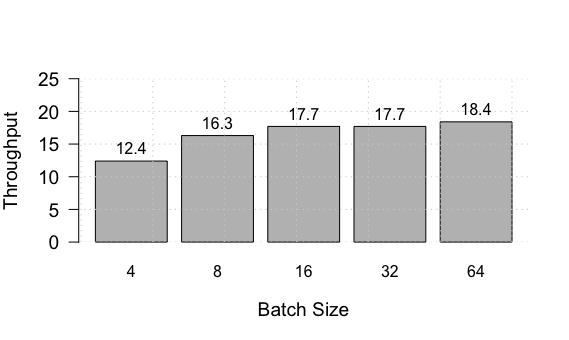
\includegraphics[width=\textwidth]{wgrid_figure3c.png}
		\caption{Throughput (in images/sec) -- 4 workers}
		\label{fig:singlenodethroughput4w}
	\end{subfigure}
			\begin{subfigure}[t]{0.45\textwidth}
				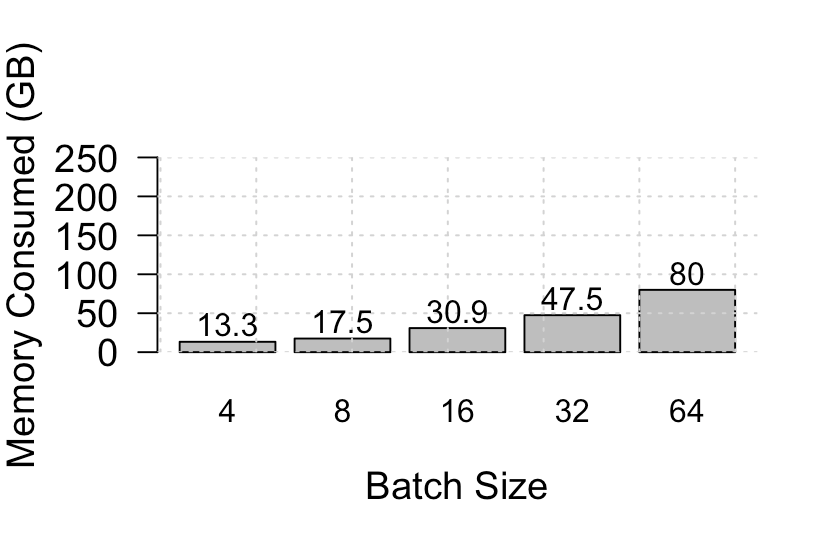
\includegraphics[width=\textwidth]{wgrid_figure3b.png}
				\caption{Memory (in GB) -- 1 worker}
				\label{fig:singlenodememutil1w}
			\end{subfigure}
			\begin{subfigure}[t]{0.45\textwidth}
				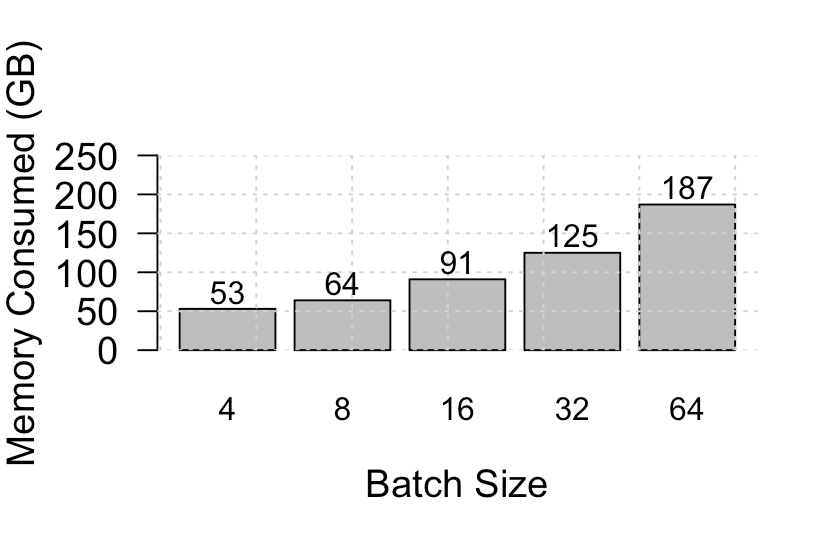
\includegraphics[width=\textwidth]{wgrid_figure3d.png}
				\caption{Memory (in GB) -- 4 workers}
				\label{fig:singlenodememutil4w}
			\end{subfigure}
			\caption{\label{fig:multiworker}
				\textsf{Throughput (in images/second) and memory utilized (in GB) with batch sizes 4 to 64 for 1 and 4 training workers respectively (a and b) on a single 2S Intel\textregistered{} Xeon\textregistered{} Gold 6148 processor with Dataset A.}}
		\end{figure}

		\begin{figure}[h!]
			\centering
			\resizebox{0.95\columnwidth}{1.2in}{
				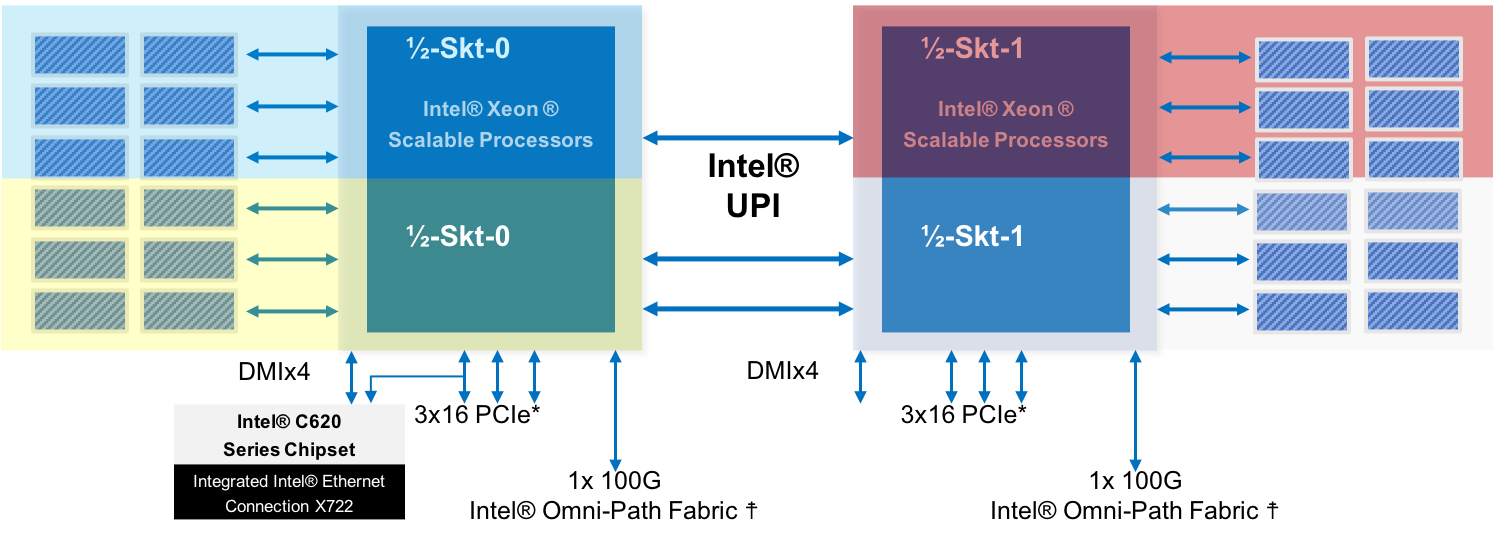
\includegraphics{twosocket.png}
			}
			\caption{\textsf{Two socket Intel\textregistered{} Xeon\textregistered{} Gold 6148 processor NUMA configuration}}
			\label{fig:multisocket}
		\end{figure}
	
\noindent Second, for all batch size configurations, CPU utilization was low meaning the cores were under-utilized. Upon further investigation with system profile, we found 1) there were lots of context switches and 2) processes or threads assigned to one CPU socket are accessing data from the other CPU socket including a long latency hop over the socket-to-socket interconnect. This led to the discovery that using multiple workers or instanes per socket can yield faster TTT. The essence of using multiple workers in a single CPU is to affinitize tasks to cores and bind their memory allocation to local non-uniform memory access (NUMA) banks as shown by the shaded rectangles in \autoref{fig:multisocket}. Memory binding is key here as it avoids redundant fetches over the interconnect to the memory channels of the adjacent CPU socket. More detailed analysis of multiple workers or instances in training and inference are described in detail by Saletore and colleagues, in \cite{Saletore2018}. \\

\noindent While the authors mention that instantiating multiple workers boosts performance, they do not specify the optimal number of workers, which can depend on a variety of factors, including the neural network topology being trained, CPU micro-architecture, and characteristics of the input data. To find the best combination of workers and local batch size per worker, we experimented with 1, 2, 4 and 8 workers per CPU. In this case, 4 workers with 8 local mini-batch size resulted in the highest throughput per node. A detailed analysis of throughput and memory utilization for 4 workers is shown in Figure \ref{fig:multiworker} \subref{fig:singlenodethroughput4w} and Figure \ref{fig:multiworker} \subref{fig:singlenodememutil4w}, respectively. Note that throughput with batch sizes of 64, 128, or 256 was higher than with a batch size of 32, but these configurations did not converge any faster.
	\end{subsection}
	\begin{subsection}{Scaling out TTT on 8 Servers with Dataset A}
		\label{sec:scaleout_dataset1}
\noindent After determining the number of workers per node, we deployed the training on 8 nodes with 4 workers per node. We used the MPI Allreduce mechanism in Uber's Horovod library to synchronize the gradients. As indicated in \autoref{fig:mcnn}, the model size is 162MB which was the size of the gradients exchanged between the workers per iteration. Due to this high bandwidth requirement, we used a 100Gbps Intel\textregistered{} Omni-Path Fabric (Intel\textregistered{} OP Fabric). Note here that each layer of M-CNN calls \emph{Horovod\_Allreduce}, resulting in a large variation in the MPI negotaition calls. The MPI negotiation times range between 450ms and 858ms. The final time to convergence on 8 nodes is shown in \autoref{fig:8node}. \autoref{fig:8node}\subref{fig:loss8node} shows the training loss over epochs and \autoref{fig:8node}\subref{fig:accuracy8node} shows the time to achieve state of the art top-1 and top-5 accuracy on Dataset A. From the results, we see that using 8x more hardware resources we were able to scale TTT by 6.6X. With Dataset A, this means a TTT of 31 minutes which is well within our target of one hour. This also encouraged us to explore a larger dataset we would need more hardware resources. Hence, we chose Dataset B with 313,282 images. The experiment results follow in the next section.

\begin{figure}
	\begin{subfigure}[b]{0.5\columnwidth}
		\centering
		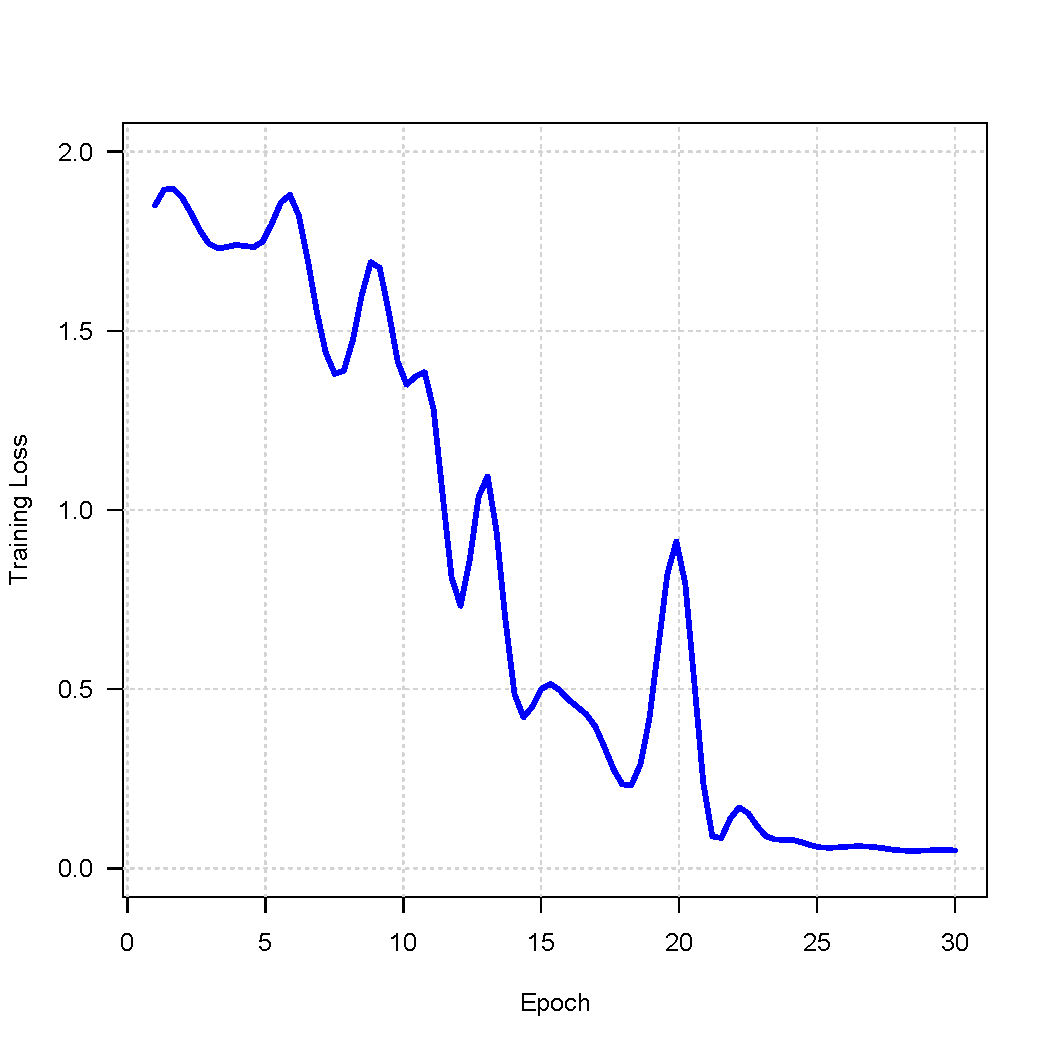
\includegraphics[height=2.5in]{figure5a.pdf}
		\caption{Training loss}
		\label{fig:loss8node}
	\end{subfigure}
	\begin{subfigure}[b]{0.5\columnwidth}
		\centering
		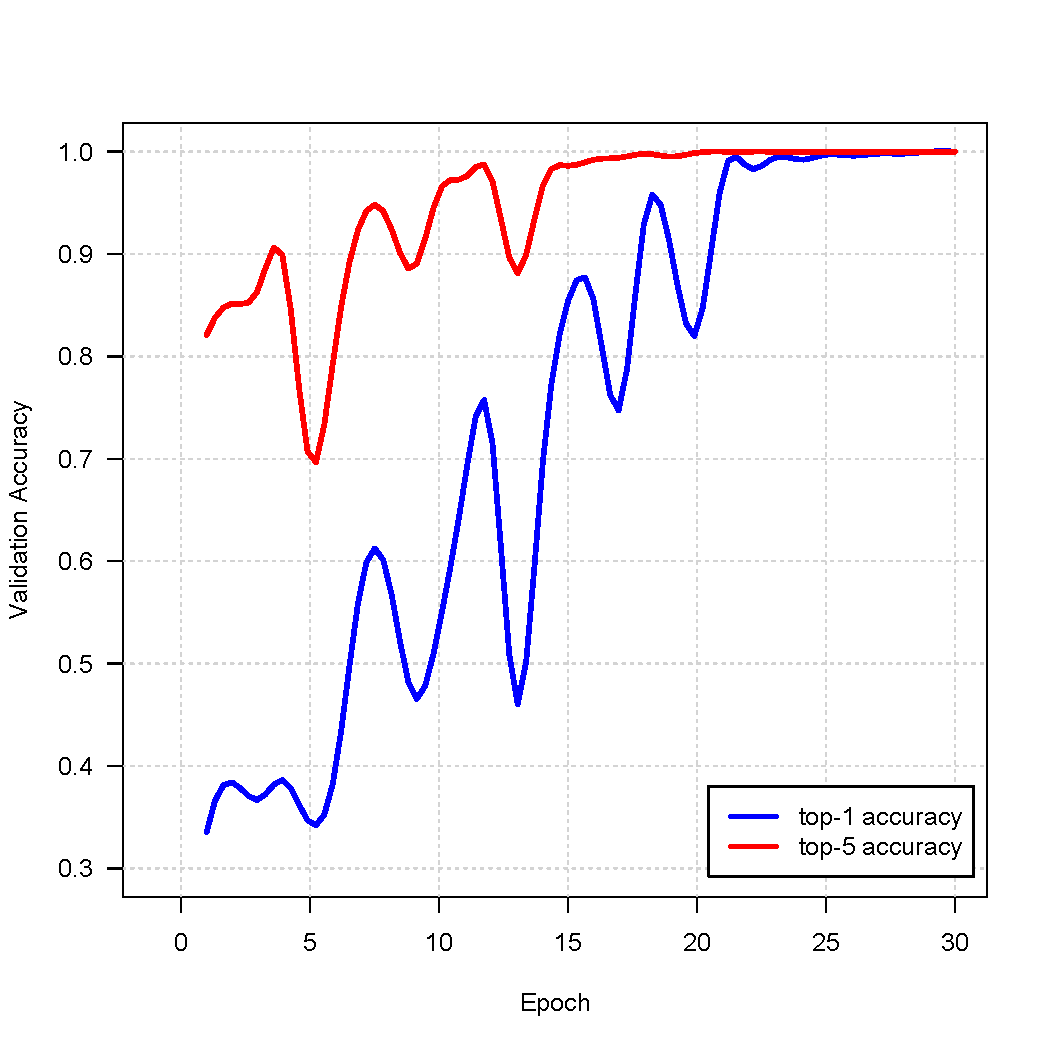
\includegraphics[height=2.5in]{figure5b.pdf}
		\caption{Validation accuracy}
		\label{fig:accuracy8node}		
	\end{subfigure}
	\caption{\label{fig:8node}%
		\textsf{Training loss, top-1 and top-5 accuracy of M-CNN model with Dataset A in 30 epochs on 8x 2S Intel\textregistered{} Xeon\textregistered{} Gold 6148 processors connected with Intel\textregistered{} OP Fabric}}
\end{figure}

\begin{figure}
	\centering
	%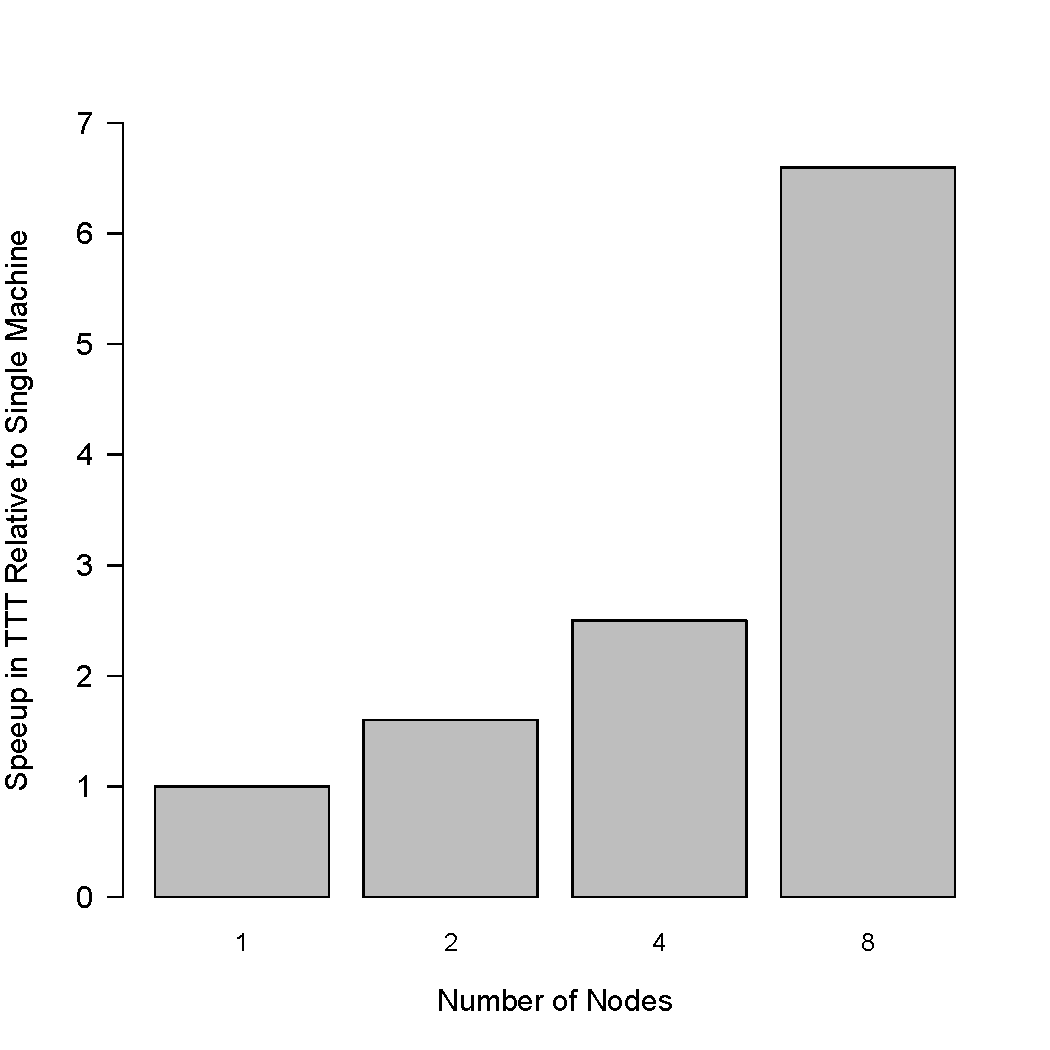
\includegraphics[width=\textwidth]{figure6.pdf}
	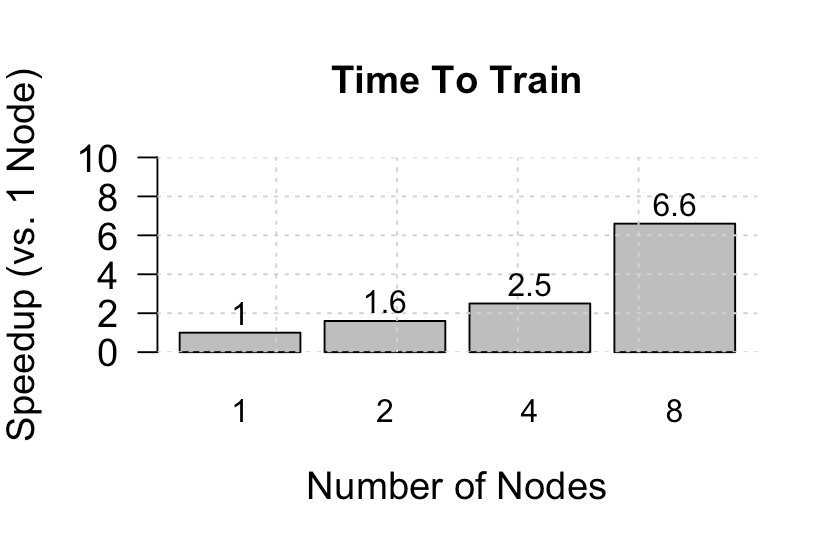
\includegraphics[width=2.5in]{wgrid_figure6.png}
	%\resizebox{0.9\columnwidth}{!}{
	%	\begin{tikzpicture}% coordinates
	%	\begin{axis}[
	%	ybar,
	%	bar width=1cm,
	%	xtick=data,
	%	symbolic x coords={1,2,4,8},
	%	nodes near coords,
	%	grid=major,
	%	major grid style={dotted},
	%	xlabel=Intel\textregistered{} 2S Xeon\textregistered{} Nodes,
	%	ylabel=Speedup in Training Time]
	%	\addplot[fill=cyan, postaction={pattern=north west lines}] plot coordinates
	%	{(1,1.0) (2, 1.6) (4, 2.5) (8, 6.6)};
	%	\end{axis}		
	%	\end{tikzpicture}}
	\caption{\textsf{Scaling M-CNN training with Dataset A from 1X to 8X 2S Intel\textregistered{} Xeon\textregistered{} Gold 6148 processors connected with 100Gbps Intel\textregistered{} OP Fabric}}
	\label{fig:scaleout_dataset1}
\end{figure}
\end{subsection}

	\begin{subsection}{Scaling out TTT on 128 Servers with Dataset B}
		\label{sec:scaleout_dataset2}
		\begin{table*}[b!]
			\begin{center}
				\caption{M-CNN Training Performance on 128 2S Intel\textregistered{} Xeon\textregistered{} Gold processors with Dataset B}
				{\renewcommand{\arraystretch}{1.5}%
					\begin{tabular}{|c|c|c|c|c|}
						\hline
						\textbf{\# of Nodes} & \textbf{\# of Epochs} & \textbf{Batch Size} & \textbf{TTT (mins)} & \textbf{Images/sec}\\
						\hline
						\hline
						1 & \centering6.6 & 128 & 960 & 30\\
						%\hline
						2 & \centering8 & 256 & 642 & 72\\
						%\hline
						4 & \centering8.7 & 512 & 320 & 141\\
						%\hline
						8 & \centering12 & 1024 & 240 & 262\\
						%\hline
						16 & \centering15.9 & 2048 & 150 & 553\\
						%\hline
						32 & \centering14.9 & 2048 & 85 & 893\\
						%\hline
						64 & \centering15 & 2048 & 61 & 1284\\
						% \hline
						128 & \centering15.2 & 2048 & 50 & 1587\\
						\hline
				\end{tabular}}
				\label{table:mcnn128nodes} 
			\end{center}
		\end{table*}
	
\noindent \autoref{table:mcnn128nodes} summarizes the 19.2X performance improvement acheived by scaling from 1 to 128 Intel\textregistered{} Xeon\textregistered{} Gold 6148 processors with Dataset B bringing TTT to 50 minutes. The second column in the table shows number of epochs when training reach 99\% top-1 accuracy and 100\% top-5 accuracy. Subsequent columns show the global mini-batch size, time to train (in minutes) and effective throughput in images/second for each node configuration. 8 training workers per node were used in these experiments as the image dimensions in Dataset B are smaller than Dataset A.\\

\noindent The key takeaway here is that updates per epoch is critical to acheive convergence. Global mini batch size determines the number of updates per epoch and M-CNN did not converge beyond global batch sizes of 2048. Hence, we maintained the global batch size to 2048 while scaling from 16 to 128 nodes -- the idea of strong scaling taken from HPC applications. As the same amount of work is increasingly divided across more CPU cores we observe diminishing returns in speedup albeit overall TTT improves. Note that our objective is to not show linear scaling here, but to see what resources will help us acheive a TTT less than one hour. \\\\
\noindent Anothe key takeaway is that large number of workers required larger number of epochs to converge. This also affects scaling. This is again an artifact of the dataset. Finally, in \autoref{fig:top1acc_dataset2}, we show the behavior of top-1 accuracy and learning rate per epoch for each of the configurations. Note here that use the linear learning rate scaling rule discussed in \autoref{sec:lr}. The learning rate is scaled according to the ratio of increase in global mini batch size. However, as shown in the \autoref{fig:top1acc_dataset2} similar to global batch size, learning rate scaling has to capped to 2048 beyond 16 nodes for the model to converge. \\\\
		\begin{figure*}[t!]
			\centering
			\begin{subfigure}[b]{0.25\textwidth}
				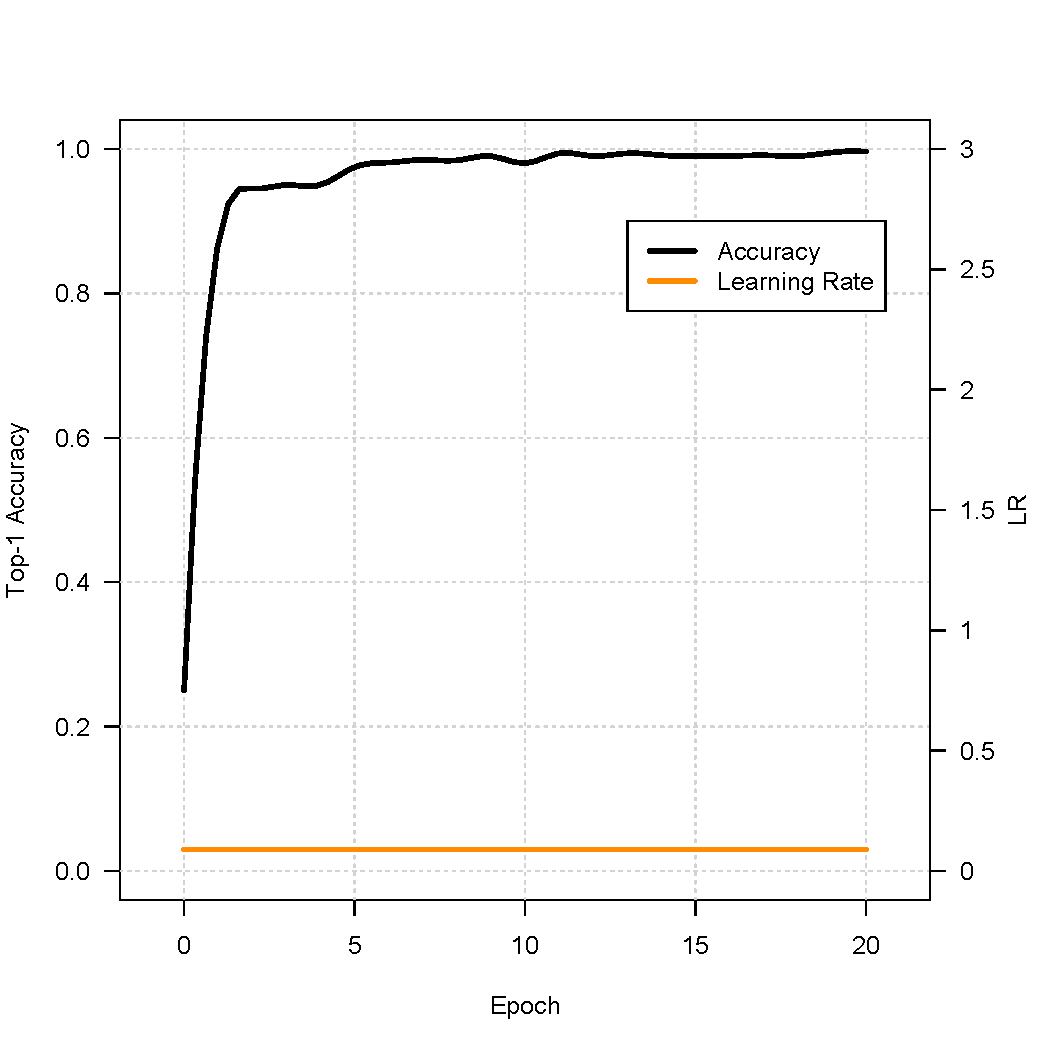
\includegraphics[width=1.5in]{figure7a.pdf}
			\caption{1 node}
			\end{subfigure}%
			\begin{subfigure}[b]{0.25\textwidth}
				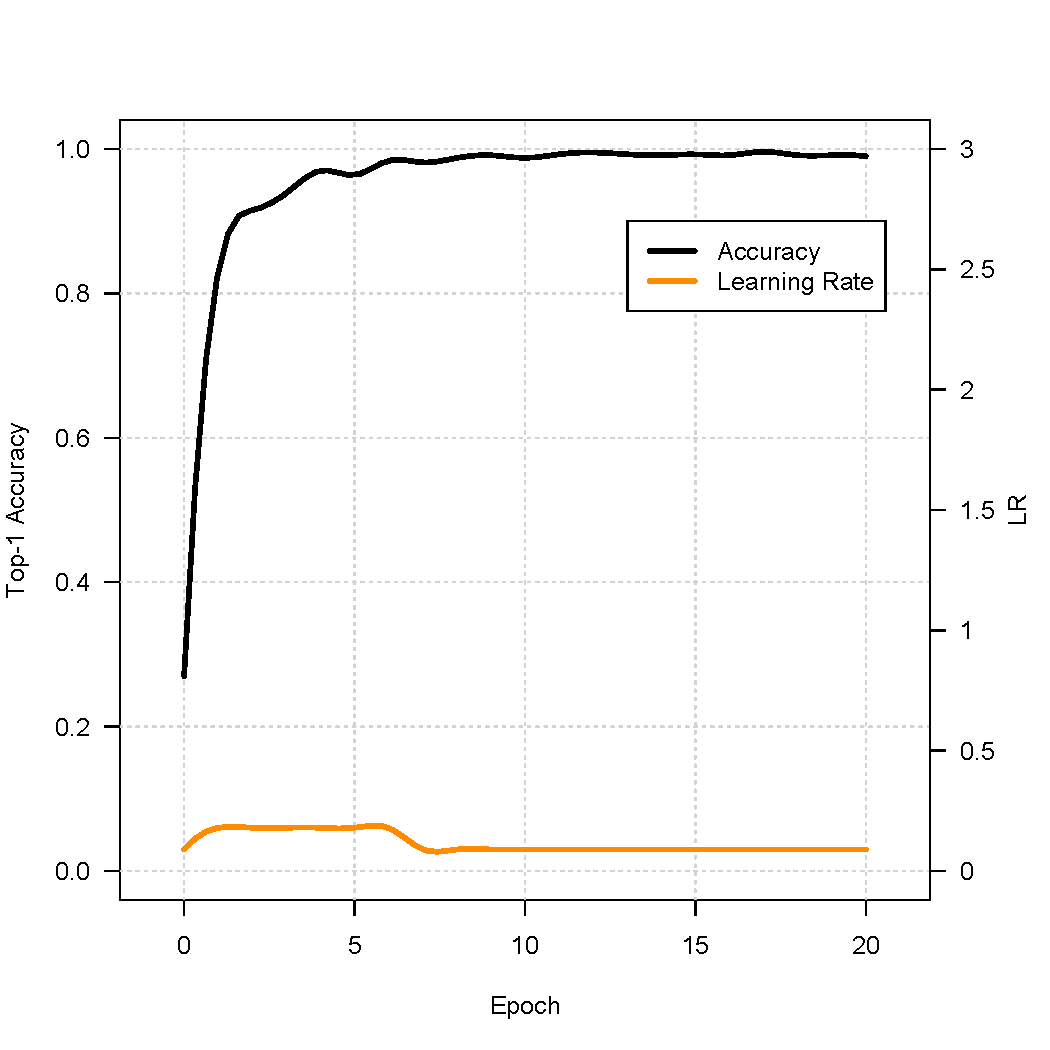
\includegraphics[height=1.5in]{figure7b.pdf}
			\caption{2 nodes}
			\end{subfigure}%
		    \begin{subfigure}[b]{0.25\textwidth}
		   		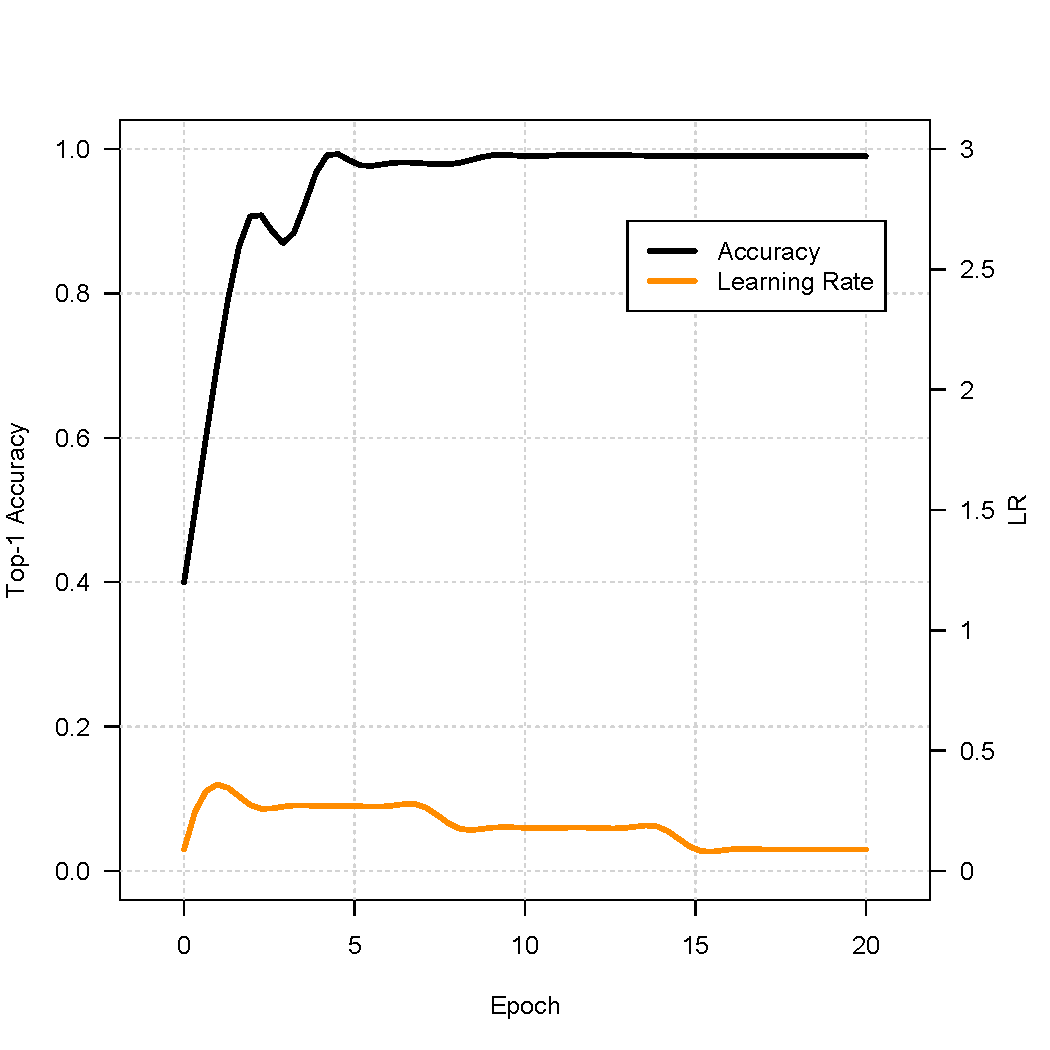
\includegraphics[height=1.5in]{figure7c.pdf}
		    \caption{4 nodes}
		    \end{subfigure}%
		    \begin{subfigure}[b]{0.25\textwidth}
		   		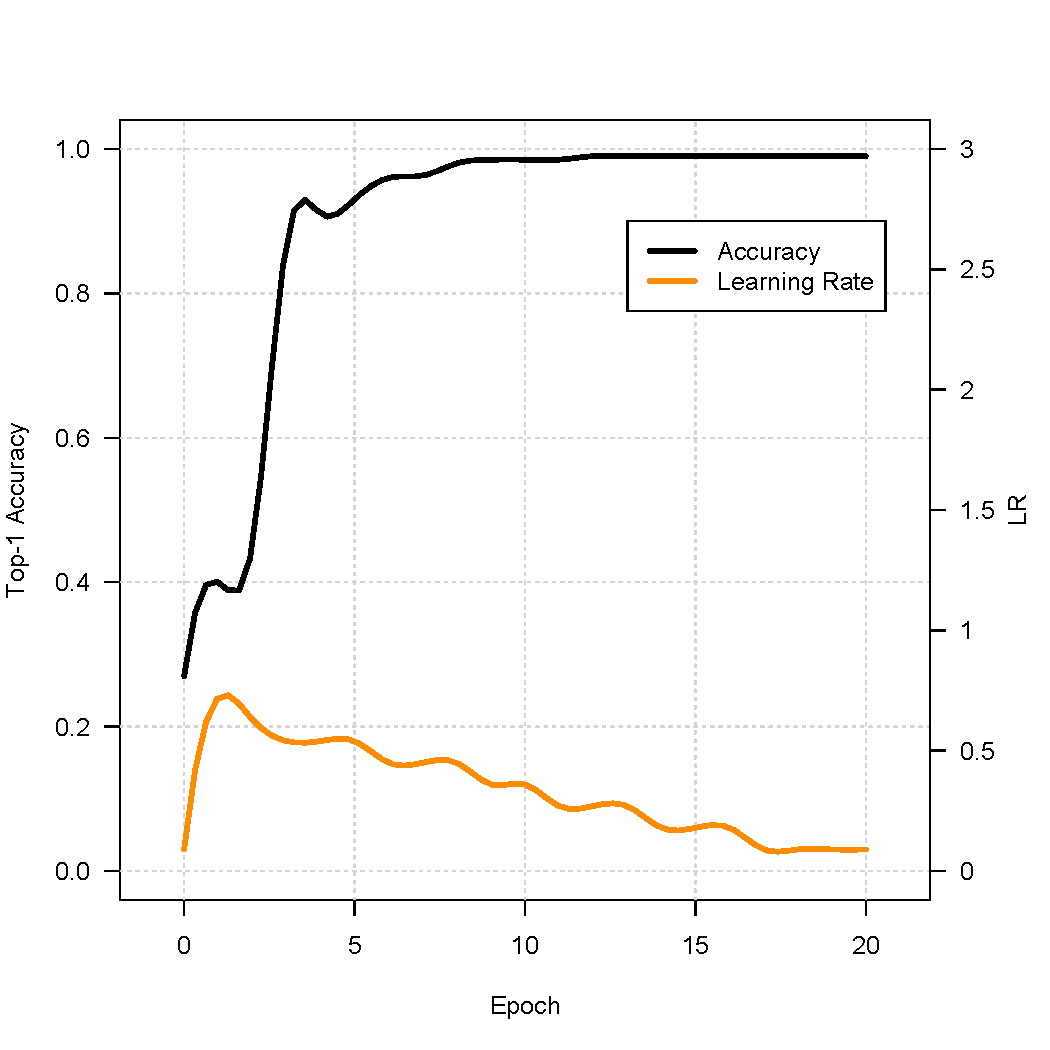
\includegraphics[height=1.5in]{figure7d.pdf}
		    \caption{8 nodes}
		    \end{subfigure}
		    \begin{subfigure}[b]{0.25\textwidth}
		    	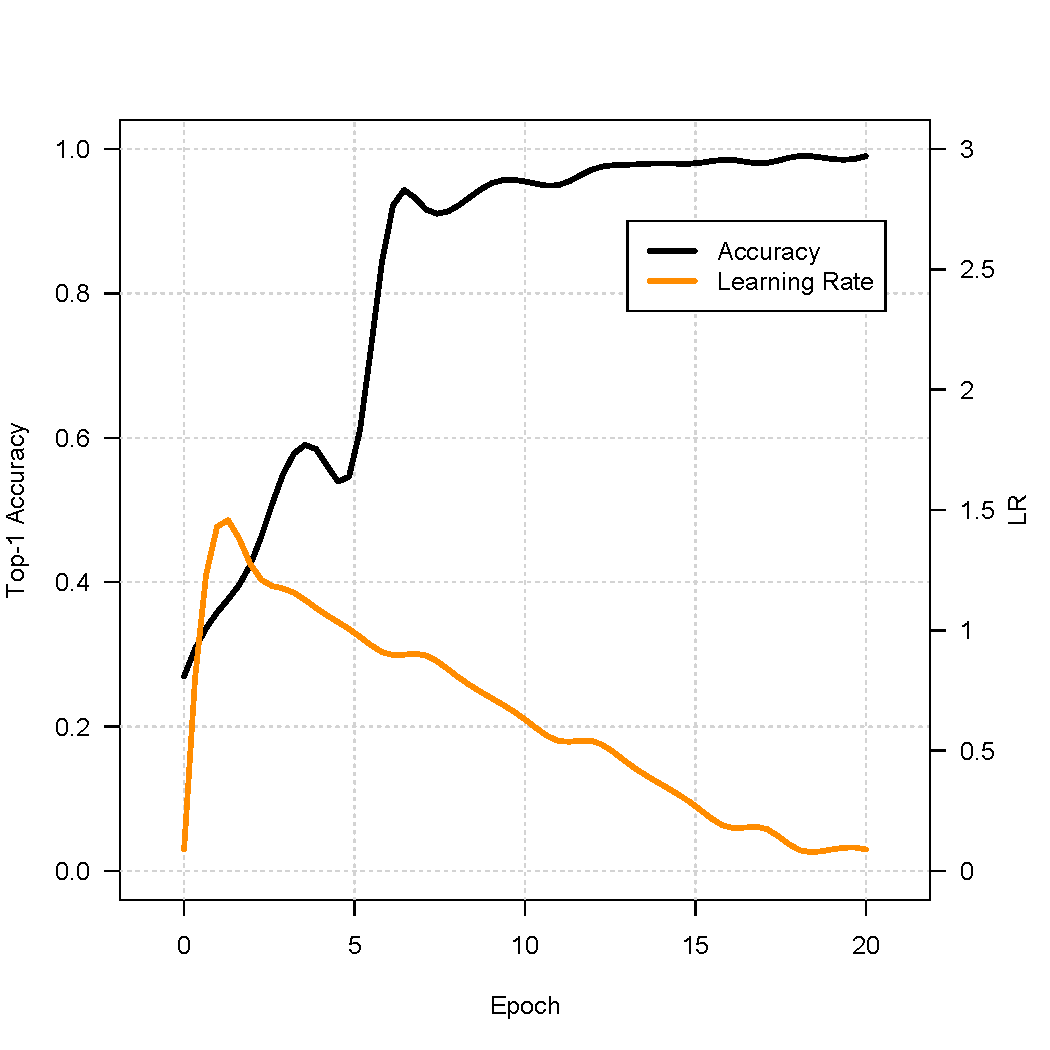
\includegraphics[height=1.5in]{figure7e.pdf}
		    \caption{16 nodes}
		    \end{subfigure}%
		    \begin{subfigure}[b]{0.25\textwidth}
		    	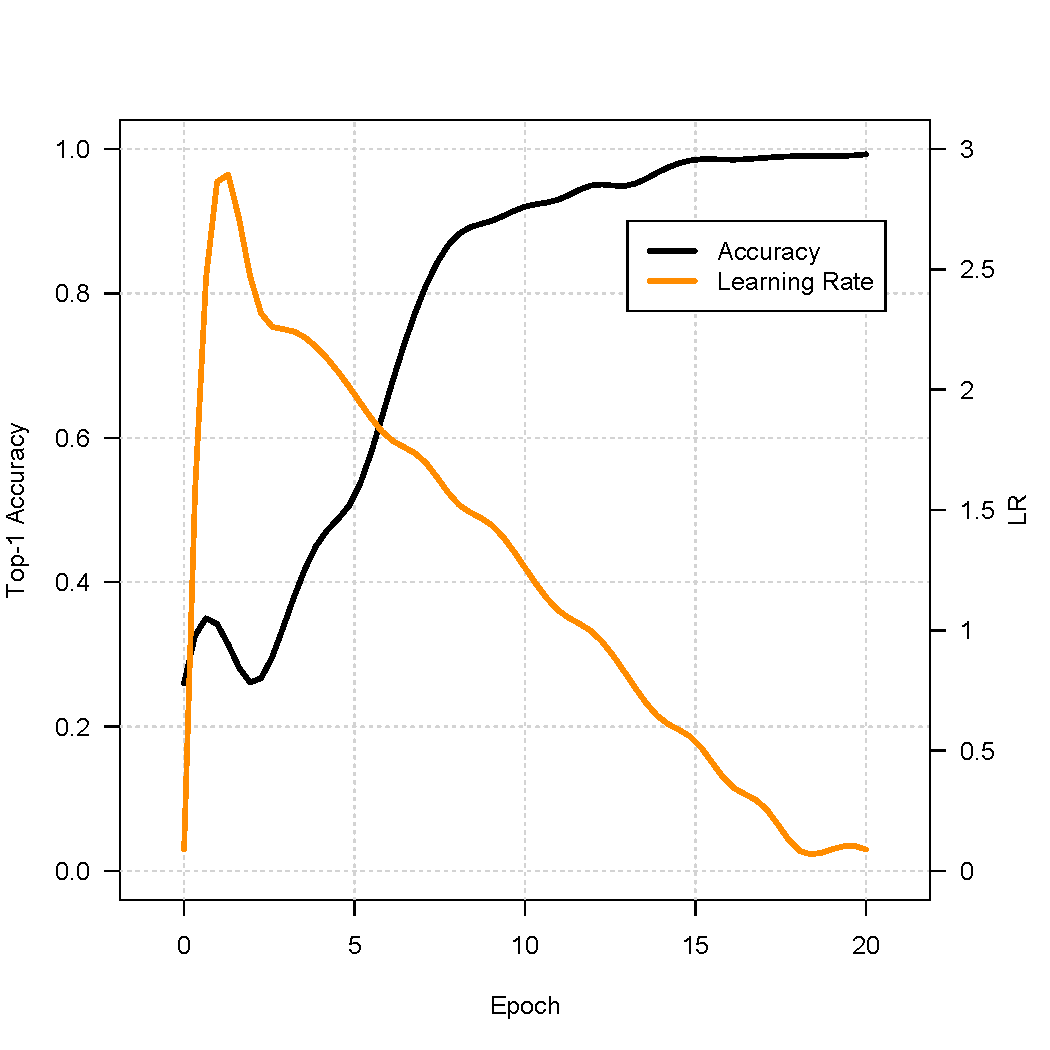
\includegraphics[height=1.5in]{figure7f.pdf}
		    \caption{32 nodes}
		    \end{subfigure}%
			\begin{subfigure}[b]{0.25\textwidth}
				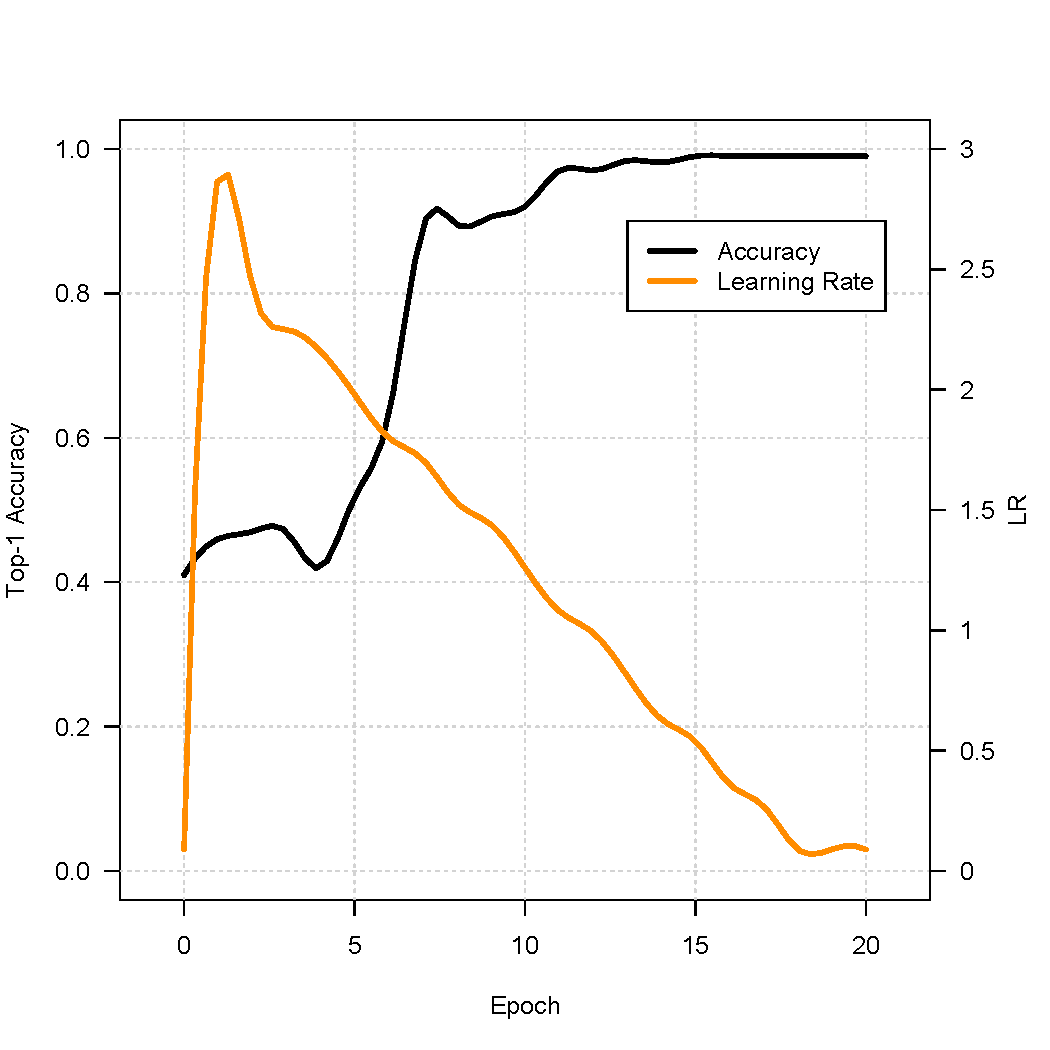
\includegraphics[height=1.5in]{figure7g.pdf}
			\caption{64 nodes}
			\end{subfigure}
			\caption{Top-1 Accuracy achieved in 20 epochs of M-CNN training and Learning Rate used on 1--64 2S Intel\textregistered{} Xeon\textregistered{} Gold processors. Dataset B is used for these experiments. Global minibatch size is capped at 2K from 16 to 64 nodes. The learning rate as shown in (f) -- (h) is also scaled only to 0.032 to achieve convergence}
			\label{fig:top1acc_dataset2}
		\end{figure*}
		\begin{figure*}
			\centering
			% \includegraphics[height=1.75in]{figure8.pdf}
			\resizebox{0.8\columnwidth}{!}{
				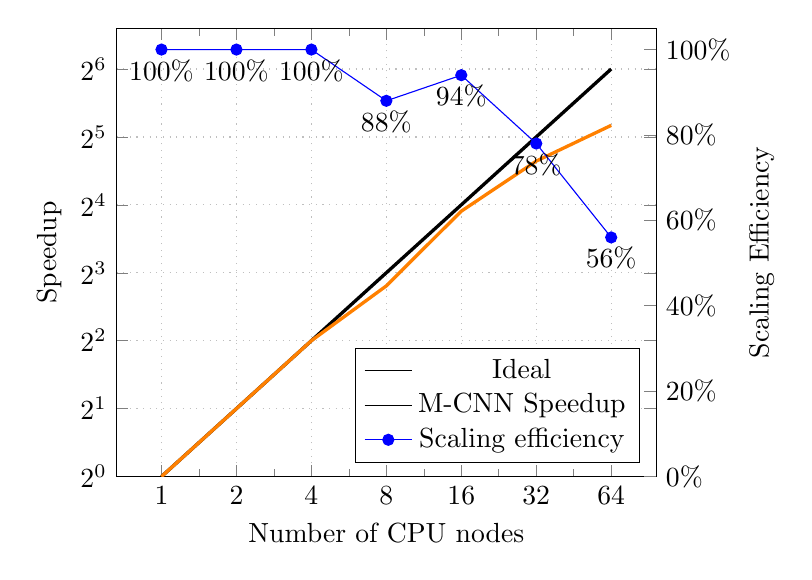
\begin{tikzpicture}
				\begin{axis}[minor tick num=1,
				xlabel=Number of CPU nodes,
				xtick=data,
				symbolic x coords={1,2,4,8,16,32,64,128},
				ymin=1,
				ylabel=Speedup,
				ymode=log,
				log basis y={2},
				grid=major,
				major grid style={dotted}]
				\addplot [black,very thick] coordinates {(1,1) (2,2) (4,4) (8,8) (16,16) (32,32) (64,64)}; %(128,128)};
				\label{plotOne}
				\addplot [orange,very thick] coordinates {(1,1) (2,2) (4,4) (8,7) (16,15) (32,25) (64,36)}; %(128,44)};
				\label{plotTwo}
				\end{axis}
		        
				\begin{axis}[
				axis y line*=right,
				axis x line=none,
				xtick=data,
				symbolic x coords={1,2,4,8,16,32,64}, %,128},
				ymin=0, ymax=105,
				ylabel=Scaling Efficiency,
				ytick=\empty,
				extra y ticks={0,20,40,60,80,100},
				extra y tick labels={0\%,20\%,40\%,60\%,80\%,100\%},
				nodes near coords={\pgfmathprintnumber\pgfplotspointmeta\%},
				nodes near coords align=below,
				every node near coord/.append style={color=black},
				legend pos=south east]
				\addlegendimage{/pgfplots/refstyle=plotOne}\addlegendentry{Ideal}
				\addlegendimage{/pgfplots/refstyle=plotTwo}\addlegendentry{M-CNN Speedup}
				\addplot [mark=*,blue] coordinates {(1,100) (2,100) (4,100) (8,88) (16,94) (32,78) (64,56)}; %(128,34)};
				\addlegendentry{Scaling efficiency}
				\end{axis}
				\end{tikzpicture}}
			\caption{Scalability of M-CNN training performance for 20 epochs on 64 2S Intel\textregistered{} Xeon\textregistered{} Gold 6148 processors. Note that global batch size is capped at 2K from 16 -- 64 nodes. Intel\textregistered{} OP Fabric, TensorFlow-1.9.0+Horovod, OpenMPI v3.0.0, 8 workers/node}
			\label{fig:20epoch_dataset2}
		\end{figure*}
\noindent Additionally, we show the scaling efficiency of M-CNN training from 1 to 64 nodes all running for 20 epochs. As shown in \autoref{fig:20epoch_dataset2} time to train efficiently scales up to 16 nodes after which capping the global mini batch size shows diminishing returns.
	\end{subsection}
\end{section}
